\documentclass[a4paper,11pt]{article}
\usepackage[utf8]{inputenc}
\usepackage{amsmath}
\usepackage{amsfonts}
\usepackage{amssymb}
\usepackage{graphicx}
\usepackage{tabularx}
\usepackage[font=scriptsize]{caption}
\usepackage[font=scriptsize]{subcaption}
\usepackage{wrapfig}
\usepackage[backend=biber]{biblatex}

\addbibresource{nn.bib}
\renewcommand\thesubsection{\alph{subsection}}


%opening
\title{One-dimensional traveling waves in neural columns}
\author{Vince Baker, advisor: Dr. Luis Cruz Cruz\\ Drexel University Department of Physics}

\begin{document}

\maketitle

\begin{abstract}
Traveling waves of neural activity in the cortex have been observed in vivo.
These traveling waves explain various features of observed cortical dynamics including spike timing variability and correlated fluctuations in neuron membrane potential.
To undertand networks of neurons as a medium for wave propagation we explore a one-dimensional network of neurons with biologically influenced models of neuron dynamics and connectivity.
We find that background stimulus reliably evokes traveling waves in networks with local connectivity between neurons.
We also observe traveling waves in fully-connected networks when a model for action potential propagation speed is incorporated.
The biological properties of the neurons influence the generation, annihilation and propagation of the traveling waves. 
Our one-dimensional model is not only useful for studying the basic properties of traveling waves in neural networks.
It also provides a simplified representation of the mini-column or micro-column structural elements that are found in the cortex.

\end{abstract}

\section{Introduction} 
Neurons in the brain that fire sequentially can spread their firings to neighboring neurons creating what has been called a traveling wave of neuron activation. 
These traveling waves have been observed in the cortex of mammalian brains as well as in vitro, and subsequently have been reproduced in silico. 
While the function of traveling waves is unknown, proposed functions include motor coordination, place field coordination in the hippocampus, and spatiotemporal processing in the visual cortex \cite{muller2018}. 

Different types of neuronal traveling waves have been studied in the literature. 
In the sleep and anesthetized states, slow and large-scale wave activity has been recorded \cite{muller2018}. 
Local-area traveling waves in the awake cortex have been observed using recent advances in optical imaging techniques using voltage-sensitive dyes \cite{wu2008}. 
Both spontaneously occurring waves and stimulus-evoked waves have been observed in the visual and auditory cortex \cite{reimer2010}\cite{muller2018}.
Traveling waves have also been observed in simulations of neural networks \cite{keane2015}.

In this work we explore the fundamental dynamics of traveling waves in networks of neurons.
We choose a physical model with one spatial dimension much longer than the other two, so that we can stuy one-dimensional traveling waves.
Our neuron dynamics are based on the Izhikevich model\cite{izhikevich2003}, allowing us to explore more complex neuron dynamics than previous work based on integrate-and-fire neurons \cite{keane2015}.
We also incorporate the action potential propagation time in our model unlike many other large-scale neural simulations.

We find that these traveling waves in one dimension can propagate in simulated neural column structures with certain properties including distance-dependent connectivity and a mix of excitatory and inhibitory neurons. 
We observe wave properties including creation from background stimulus, annihilation between waves, and a wave velocity that is determined by both the action potential propagation speed and the column topology. 

The vast majority of studies of traveling waves have focused on two-dimensional waves that spread parallel to the surface (pia) of the brain \cite{muller2018}. 
Waves traveling perpendicular to the surface have not been examined because of experimental limitations. 
However, there is no reason to believe that such traveling waves do not exist given that there are no neuronal or tissue properties preventing them from occurring. 
Gray matter in the perpendicular direction can be hundreds of microns thick with known one-dimensional structures, called micro- or minicolumns\cite{cruz2000} that can very well propagate traveling waves of neuronal activity.


\section{Methods}
We simulated the dynamics of a small neural column to explore neuron synchronization.
Our network geometry is based on the model presented in \cite{markram1998}.
An example neural column composed of 135 neurons on a unit grid spacing, 3x3 neurons wide and 15 neurons high as shown in figure \ref{fig:column_structure}.
\begin{figure}[!htb]
 \caption{Example column structure used in this research, $\lambda=2.5$,$C=1$. The left image shows the connections between neurons in the column, the color scale indicates connection length. The right image shows inter-neuron connectivity for excitatory connections (green) and inhibitoruy connections (red).}
 \label{fig:column_structure}
 \centering
   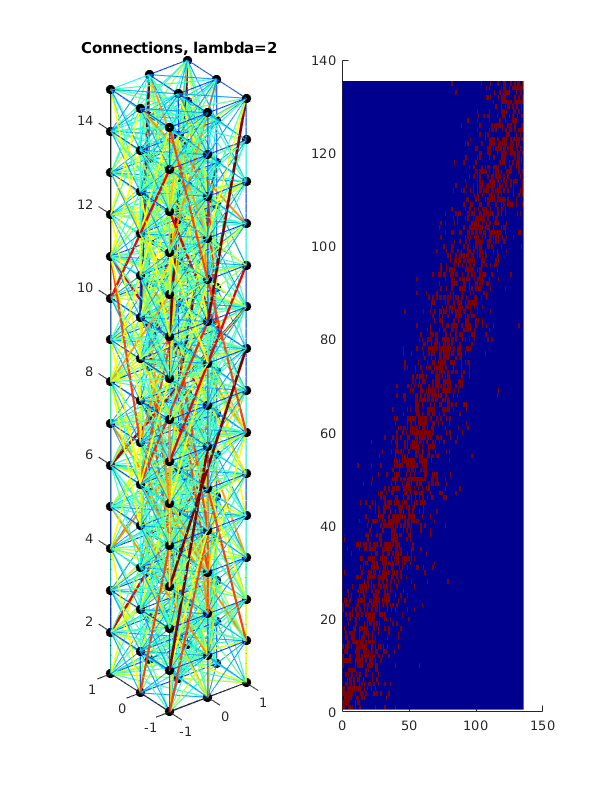
\includegraphics[width=\textwidth]{fig/lambda2}
\end{figure}
The neurons are connected with a strong local connectivity according to the distance-based connection probability:
\begin{align}\label{eq:connectivity}
 P_{a,b} &= C \times e^{-(D(a,b)/\lambda)^2}
\end{align}
Where $D(a,b)$ is the distance between neuron A and B and $\lambda$ and $C$ are parameters of the connection model.

We model the neurons using the Izhikevich model \cite{izhikevich2003} to allow us to explore the neural dynamics.
The Izhikevich model uses two coupled differential equations with two variables and four parameters:
\begin{align}
 v^\prime &= 0.04v^2+5v+140-u+I \label{eq:neuron_v} \\
 u^\prime &= a(bv-u)\\
 \text{if } &v>30: v\leftarrow c, u\leftarrow u+d
\end{align}
This is a simplified model of a two-dimensional dynamical system.
This model has been used to reproduce common neural firing patterns.
There is MATLAB code available \cite{izzy_code} that implements this neural model with fixed, single-time-step action potential propagation.
The model parameters for excitatory and inhibitory neurons are shown in Table \ref{tab:izzy_params}.
We define $\mathcal{U}\{a,b \}$ as a uniform random variable drawn on $[ a,b ] $.
\begin{table}[!h]
 \caption{Izhekevich model parameters}
 \label{tab:izzy_params}
 \centering
 \begin{tabular}{l|c|r}
  \textbf{Parameter} & \textbf{Excitatory} & \textbf{Inhibitory} \\
  \hline
  a & 0.02 & 0.02+$\mathcal{U}$(0,0.08) \\
  b & 0.2 & 0.25-$\mathcal{U}(0,0.05)$\\
  c & -65+$\mathcal{U}(0,10)^2$ & -65 \\
  d & 8-$\mathcal{U}(0,6)$& 2 \\
 \end{tabular}
\end{table}

In the Izhikevich model when a neuron fires the action potential propagates to the target neuron at the next time step.
The action potential from the firing neuron is added to the target neuron current $I$ (Eq \ref{eq:neuron_v}).
We enhanced the available MATLAB code for the Izhikevich model to incorporate a more realistic propagation model while still minimizing computational complexity.
Our model incorporates a propagation delay $\tau_{ij}=\kappa D(i,j)$ proportional to the inter-neuron distance $D(i,j)$ between neurons $i$ and $j$. 
The parameter $\kappa$ ranges from 0 (action potentials propagate to the target neuron in the next time step) to 4. 
We also model an exponentially decaying synapse response $I(t)=e^{-(\frac{t}{\sigma_s})^2}$ with a time constant of $\sigma_s=4~ms$.

The connection strengths between neurons is based on the original Izhikevich work.
The strength for connections from presynaptic neuron $i$ to postsynaptic neuron $j$ depends on whether $i$ is inhibitory or excitatory.
\begin{align}
 S_{ij}^{excitatory} &= K \times \mathcal{U}\{0,\frac{1}{2} \} \\
 S_{ij}^{inhibitory} &= K \times \mathcal{U}\{-1,0 \} 
\end{align}
The parameter K is used to adjust the overall connection strength: $K=1$ corresponds to the original model in \cite{izzy_code}. 

The current in Equation \ref{eq:neuron_v} includes all incoming stimulus from other neurons.
With our models for action potential propagation and synapse response, the total current to neuron $i$ can be written:
\begin{align}
 I_i(t) &= \sum_{j\ne i} \sum_{t^\prime_j} S_{ij}  \Theta(t-t^\prime_j-\tau_{ij})e^{-(\frac{t-t^\prime_j-\tau_{ij}}{\sigma_s})^2}
\end{align}
Where the $t^\prime_j$ are all firing times of neuron $j$ and $\Theta$ is the Heaviside step function.

The current in Equation \ref{eq:neuron_v} also includes any stimulus applied as part of the experiment.
We perform experiments using both a uniform background stimulus and a step stimulus.
Our model for uniform background stimulus to a neuron $i$ depends on whether $i$ is inhibitory or excitatory, following Izhikevich's original model.
The uniform background stimulus is:
\begin{align}
 I_i^{excitatory} &= M \times \mathcal{U}\{0,1 \} \\
 I_i^{inhibitory} &= \frac{2}{5} M \times \mathcal{U}\{0,1 \}
\end{align}
The parameter $M$ is used to adjust the overal strength of the stimulus, $M=1$ corresponds to the original model in \cite{izzy_code}.

A step stimulus is used when measuring the speed of a traveling wave.
The step stimulus is applied uniformly to neurons in the lowest 5 layers of the column.
The stimulus starts at $t=20~ms$ and lasts for $20~ms$ during which the affected neurons receive a constant current input of strength 5.
This generates a single traveling wave with a determined start time, simplifying the propagation velocity measurement.

We capture the firing events from all neurons in each simulation.
We then perform a spatial clustering operation to identify spatiotemporal regions with a high firing density.
This clustering operation removes random background firing activity.
We then identify and label the traveling wave structures that evolve over time as shown in Figure \ref{fig:wave_analysis}.
\begin{figure}[!htb]
 \centering
 \begin{subfigure}{0.33\textwidth}
  \centering
  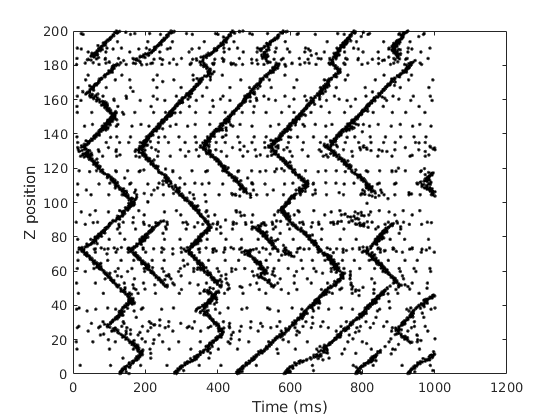
\includegraphics[width=\textwidth]{fig/2x2_firings}
 \end{subfigure}%
 \begin{subfigure}{0.33\textwidth}
  \centering
  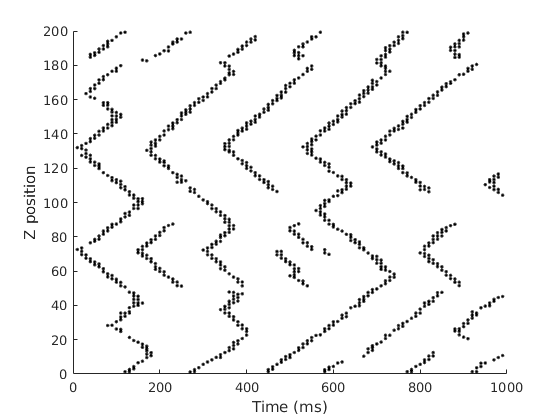
\includegraphics[width=\textwidth]{fig/2x2_density_filter}
 \end{subfigure}%
 \begin{subfigure}{0.33\textwidth}
  \centering
  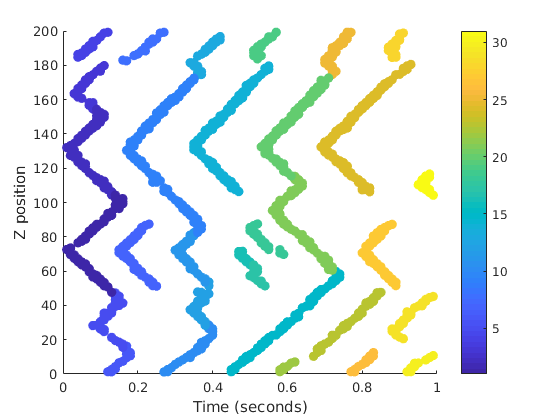
\includegraphics[width=\textwidth]{fig/2x2_wave_IDs}
 \end{subfigure}%
 \caption{Wave processing. The raw firing events (left) are filtered in time and position (center) to remove background firing events. The individual waves are then labeled with unique numbers (right, wave numer shown as color scale).}
 \label{fig:wave_analysis}
\end{figure}

Several useful measurements can be extracted from the labeled wave data, including the wave start positions and wave propagation speed.
We define the ``wave firing fraction`` as the fraction of the neuron firing events (Figure \ref{fig:wave_analysis}, left) that are associated with the labeled traveling waves.

Simulations are run with a $0.5~ms$ time step except where noted.
The traveling wave behavior looks qualitatively similar at time steps from $1~ms$ down to $10~\mu s$ (Figure \ref{fig:time_step}).
\begin{figure}[!htb]
 \centering
 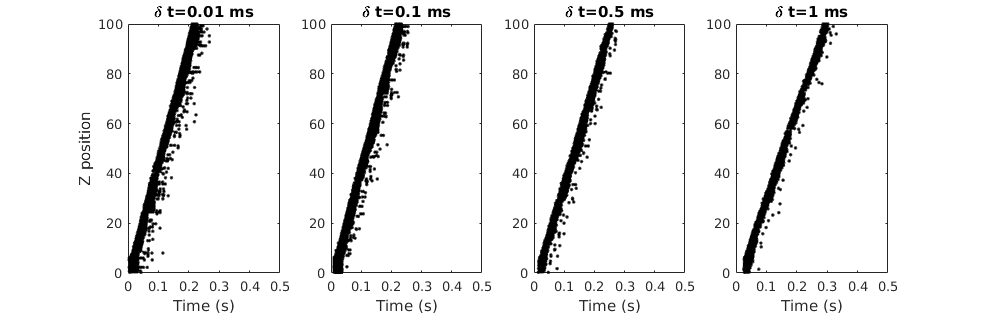
\includegraphics[width=\textwidth]{fig/TimeStepEffect}
  \caption{A traveling wave experiment at 4 different time scales. The qualitative behavior is the same.}
 \label{fig:time_step}
\end{figure}


\section{Results}
The results are organized as a series of experiments into traveling waves.
We first examine the connectivity between the neurons and find traveling waves for columns with local connectivity (\ref{sub:connectivity}).
We then examine the impact of action potential propagation delay, finding that traveling waves are supported in fully-connected columns when the propagation delay is proportional to distance (\ref{sub:delay}).
We find that the excitatory/inhibitory balance plays a role in traveling wave propagation and determines the character of column activity (\ref{sub:ei_balance}).
Wave propagation speed is investigated as a function of the action potential propagation speed and column topology, and we find that wave propagation speed is proportional to action potential propagation speed and column cross-section (\ref{sub:propagation_speed}).
Finally, we investigate the initiation of traveling waves from a uniform background stimulus and determine why a given column has preferential sites for wave initiation (\ref{sub:wave_initiation}).

\begin{table}[!htb]
 \caption{Model parameters used in the experiments in each subsection}
 \label{tab:experiment_params}
 \centering
 \begin{tabularx}{\textwidth}{l | X | c | c | c | c | c | r}
  \textbf{Section} & \textbf{Topology} & \textbf{$\lambda$} & \textbf{E/I} & \textbf{M} & \textbf{K} & \textbf{$\kappa$} \\
  \hline
  Baseline & $2x2x100$ & $2.5$ & $80\%$ & $5$ & $5$ & $1$ \\ 
  a & $2x2x100$ & $2.5$ & $80\%$ & $5$ & $\textbf{2-6}$ & $1$ \\ 
  b & $2x2x100$ & $\infty$ & $80\%$ & $5$ & $5$ & $\textbf{0,1}$ \\ 
  c & $2x2x100$ & $2.5$ & $\textbf{0-100}\%$ & $5$ & $5$ & $1$ \\ 
  d & $\textbf{(2x2,2x3,3x3)x100}$ & $2.5$ & $80\%$ & $5$ & $5$ & $\textbf{1-5}$ \\ 
  e & $2x2x50$ & $2.5$ & $\textbf{80\% , 99+\%}$ & $5$ & $5$ & $1$ \\ 
 \end{tabularx}
\end{table}

We first present a baseline experiment with uniform background stimulus to illustrate wave behavior. 
The firing events in the experiment are plotted in Figure \ref{fig:baseline}.
We note the visually well-defined traveling waves in the column, with waves being consistently initiated from approximate column positions 15, 32, 52, 70 and 90.
The waves propagate until they interact with another traveling wave or reach the ends of the column.
We observe that traveling waves annihilate each other when they meet.
The annihilation effects can be explained by the refractory period of the neurons.
Neurons that are activated by one traveling wave will be hyperpolarized and less likely to fire if another traveling waves arrives within a short time period.
\begin{figure}[!ht]
 \centering
 \caption{Baseline traveling wave experiment with uniform stimulus.}
 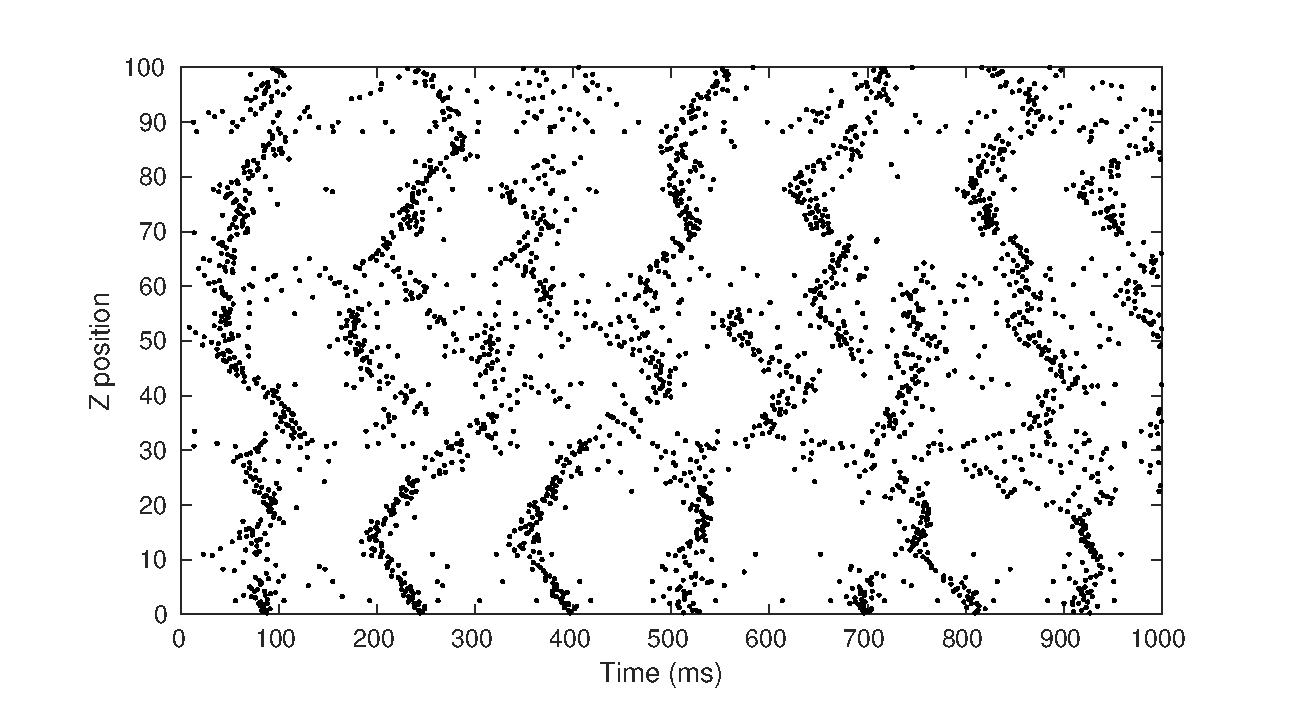
\includegraphics[width=\textwidth]{fig/baseline}
 \label{fig:baseline}
\end{figure}

\subsection{Connectivity} \label{sub:connectivity}
We first investigate the impact of connectivity on traveling wave formation.
We varied the connection strength parameter $K$ and observed the conditions under which uniform background stimulus would produce traveling waves.
We performed 100 simulations each of values of $K$ from $3$ to $12$ and determined the wave firing fraction as described in methods (Figure \ref{fig:conn_fraction}).
Below $K=3.5$ no traveling waves are detected.
We observe the transition around $K=5$ where traveling waves are observed but most of the firing events are still random.
The wave firing fraction is porportional to $K$, indicating that traveling waves dominate the firing activity as the neurons become more strongly connected.
At $K>11$ more than $90\%$ of the firing events are part of a traveling wave.
\begin{figure}[!ht]
 \caption{Traveling waves emerge around $K=5$. As the connection strength increases the traveling waves dominate all firing events in the column.}
 \centering
   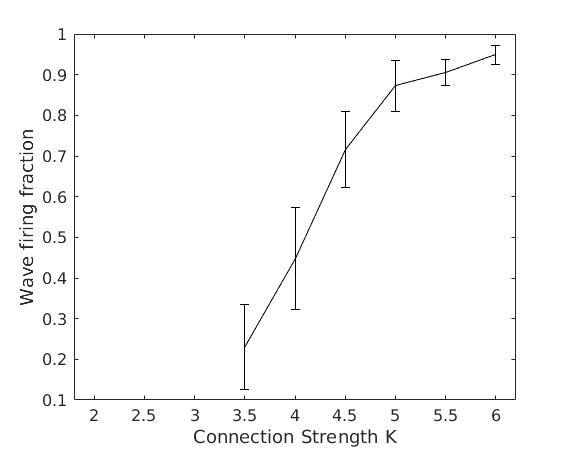
\includegraphics[width=\textwidth]{fig/ConnectionStrengthWaveFraction}  
 \label{fig:conn_fraction}
\end{figure}

\subsection{Delay} \label{sub:delay}
To investigate the impact of delay we simulate a column with complete connectivity corresponing to $\lambda \rightarrow \infty$: all neurons are connected with probability 1 to all other neurons.
This is analogous to the original Izhikevich simulation \cite{izzy_code} that demonstrated synchronized firing in a completely connected neural field with random background stimulus.
We first simulated the column with a fixed action potential propagation delay of $1~ms$ regardless of inter-neuron distance.
The result was highly synchronized simultaneous firing among all neurons in the column.
We then incorporated our distance-dependent action potential propagation with the $\kappa$ parameter set to 1.
The firing is still highly synchronized, but traveling waves are now evident (Figure \ref{fig:delay_waves}).
This demonstrates that one dimensional traveling waves can emerge from fully-connected networks if the propagation time is proportional to the inter-neuron distance.
\begin{figure}[!ht]
 \caption{Left: with global connectivity and no action potential propagation delay, the entire structure shows synchornized firing events. Right: With an action potential propagation delay, traveling wave behavior is observed.}
 \centering
   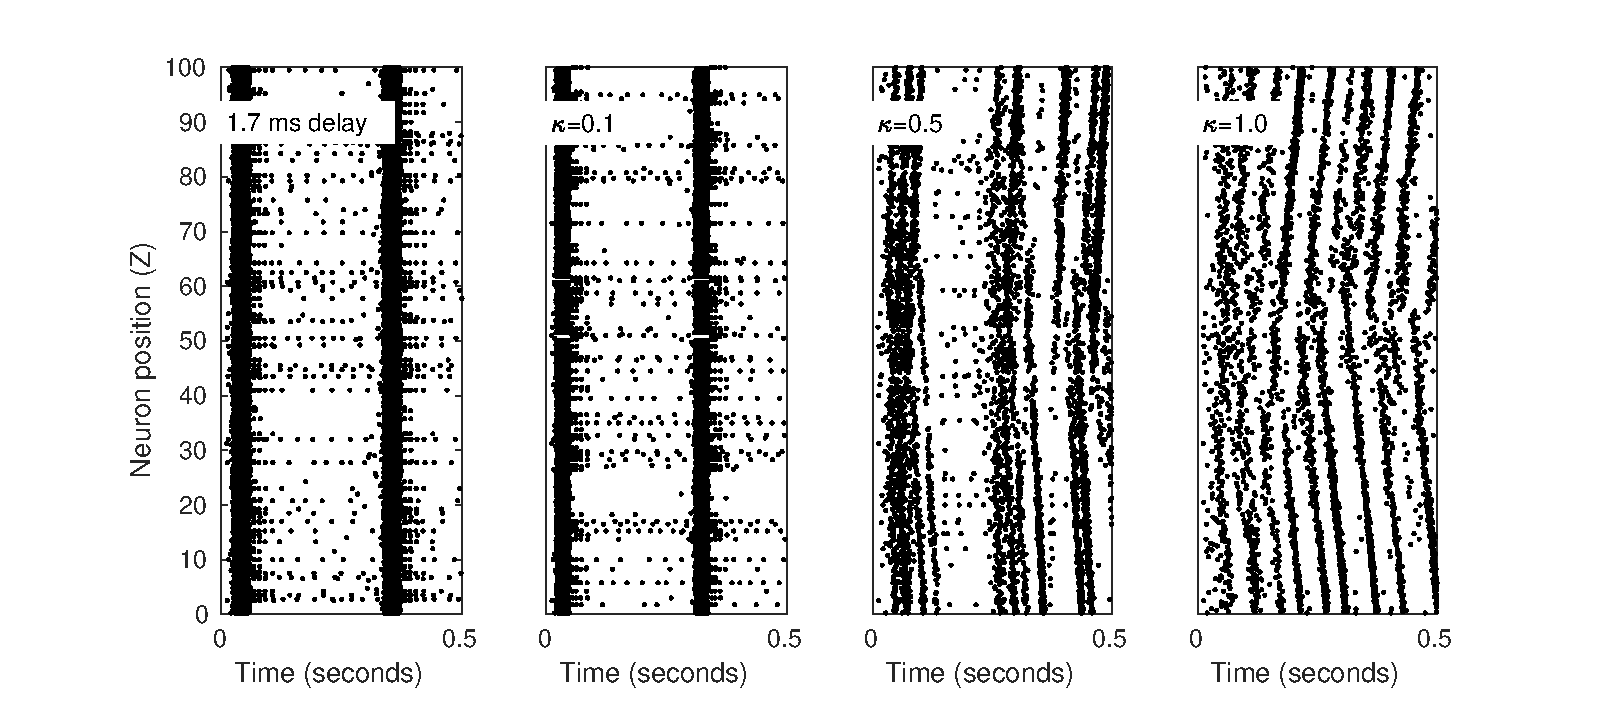
\includegraphics[width=\textwidth]{fig/DelayWaves}  
 \label{fig:delay_waves}
\end{figure}
Previous work (\cite{ermentrout2001}, Figure 1) classifies several architectures for apparent traveling waves in the cortex.
One architecture, ''Delayed Excitations from a Single Oscillator``, is a periodic source driving a sequence of excitable neurons with increasing time delays, but no connectivity between the neurons.

\subsection{Excitatory/Inhibitory Balance} \label{sub:ei_balance}
The excitatory/inhibitory balance is known to have a significant impact on neural network dynamics \cite{keane2015}. 
In our model we do not observe traveling waves if less than $40\%$ of the neurons are excitatory.
As the fraction of excitatory neurons increase we observe traveling wave patterns emerge from the background firing events.
As the excitatory fraction increases more of the firing events occur within waves structures (Figure \ref{fig:excitatory_effect}).
When all neurons are excitatory the traveling waves are the dominant mode of firing, with substantially all of the firing events contained within traveling waves. \\
\begin{figure}[!htb]
 \caption{Excitatory/inhibitory balance effect on traveling waves.. 
	  For columns with $<40\%$ excitatory neurons no waves are observed.
	  As the excitatory fraction approaches 1 nearly all firing events are part of traveling waves.
	  Error bars are 1 $\sigma$, 100 trials per measurement.
	  }
 \label{fig:excitatory_effect}
 \centering
   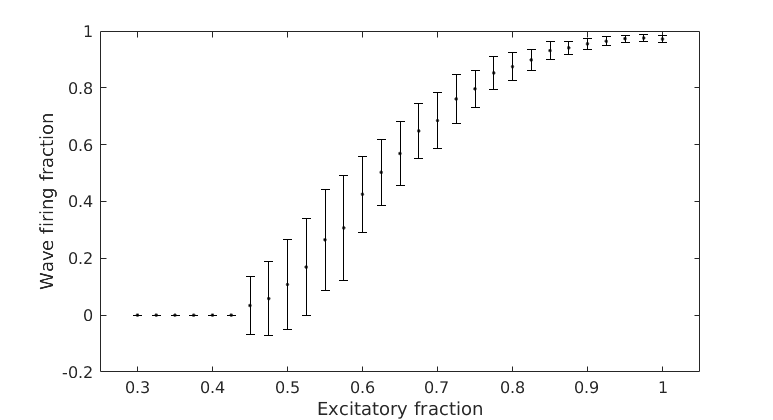
\includegraphics[width=0.5\textwidth]{fig/ExcitatoryWaves}
\end{figure}

\subsection{Propagation speed} \label{sub:propagation_speed}
To examine the velocity of the traveling waves we performed 50 velocity for measurements for two parameters of interest.
We varied the propagation delay constant $\kappa$ from (1 to 4) and the cross section of the column (2x2, 2x3, 3x3).
The results are shown in Figure \ref{fig:delay_topology}.
\begin{figure}[!htb]
 \caption{Wave speed is inversely proportional to $\kappa$ as expected. Wave speed also increases with the column cross-section.Mean values with $1\sigma$ error bars, 50 trials per measurement.}
 \label{fig:delay_topology}
 \centering
   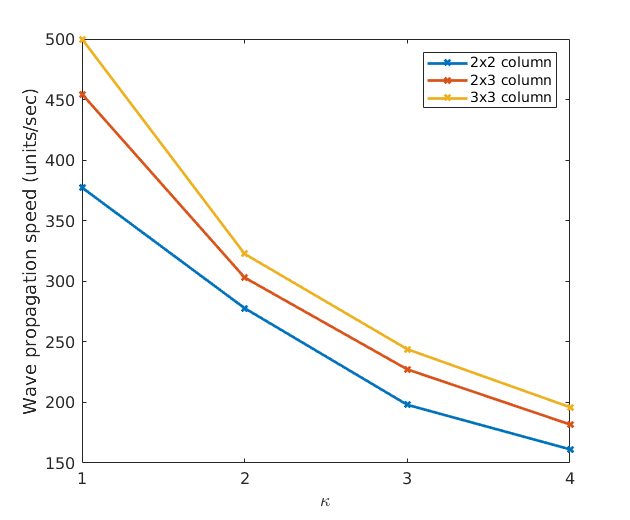
\includegraphics[width=0.75\textwidth]{fig/WaveSpeed_DelayTopology}
\end{figure}

We see that both the delay constant and the column topology influence the propagation speed.
Increasing the inter-neuron action potential delay slows the traveling wave propagation.
Waves travel faster in columns with larger cross-sections. 

\subsection{Wave Initiation and Density} \label{sub:wave_initiation}
We have observed preferential wave initiation sites in our experiments.
We hypothesize that these preferential initiation sites are created by neurons with low firing thresholds that are easy to excite.
In the Izhikevich model, inhibitory neurons can have a lower firing threshold than excitatory neurons, modeling the behavior of real inhibitory neurons in the cortex\cite{gibson2009}.
The $b$ parameter in the Izhikevich model sets the firing threshold of the individual neurons.
Neurons with higher $b$ parameter are easier to excite and therefore more likely to fire.
Per Table \ref{tab:izzy_params} excitatory neurons all have a $b$ parameter of $0.2$, while inhibitory neurons have $b$ parameters in the range $0.2-0.25$.
This indicates the preferential wave initiation sites would be due to low-threshold spiking (LTS) inhibitory neurons \cite{izhikevich2003}.
It may seem counter-intuitive that firing activity from an \underline{inhibitory} neuron would generate traveling waves.
In fact, postinhibitory rebound spiking is observed in both cortical neurons \cite{ascoli2010} and the Izhikevich model of neuron dynamics \cite{izhikevich}.

In general only some of the neurons in the column will fire when a wave passes.
We observed that a single traveling wave can have regions of higher or lower total firing activity, which we term firing density.
An example measurement of the firing activity in a single traveling wave is shown in Figure \ref{fig:wave_density}.
\begin{figure}[!htb]
 \caption{Density of firing events in a traveling wave initiated from a step stimulus. The traveling wave is shown on the left, a histogram of firing events by position is shown on the right.}
 \label{fig:wave_density}
 \centering
   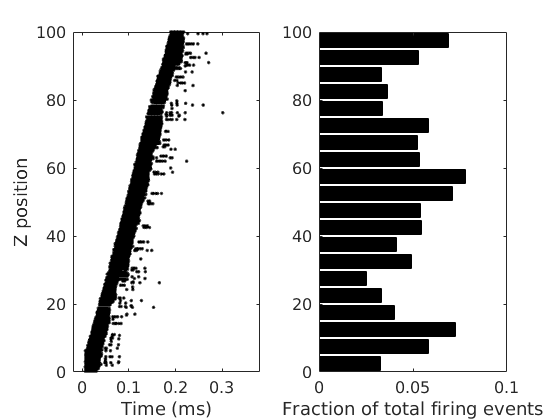
\includegraphics[width=0.75\textwidth]{fig/ImpulseWaveDensity}
\end{figure}

The wave initiation sites and wave density of the same column are shown in figure \ref{fig:initiation_density}.
This visually illustrates that the preferential firing sites tend towards lower firing density in the single wave experiments.
\begin{figure}[!htb]
 \caption{Wave initiation (left) and wave density (right) for the same column.}
 \label{fig:initiation_density}
 \centering
   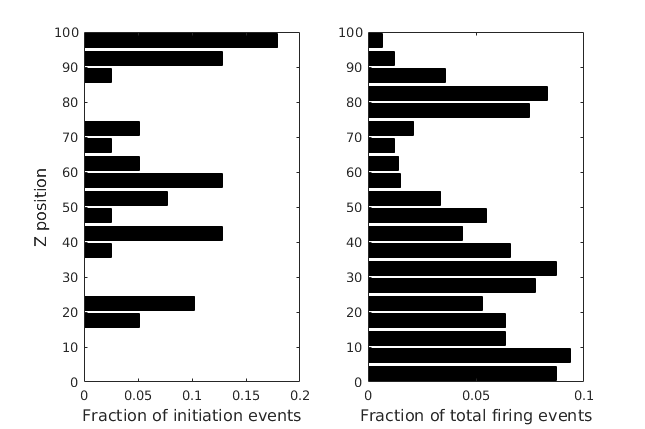
\includegraphics[width=0.75\textwidth]{fig/InitiationCorrelationHistogram}
\end{figure}

To test this hypothesis we create 100 columns, applied both uniform background stimulus and step stimulus to each column, and measured the correlation between wave initiation and firing density at the positions of the column.
Although there is substantial variation between columns we measure a consistently negative correlation coefficient (mean $-0.18$, standard deviation $0.20$).
We expect that the lower firing density is caused by the low-threshold inhibitory neurons at those sites that are responsible for generating traveling waves under uniform background stimulus.

To demonstrate that the low-threshold spiking inhibitory neurons are responsible for both generating traveling waves under background stimulus and suppressing firing activity inside a single traveling wave we performed a final experiment.
We created a column with entirely excitatory neurons except for a single LTS inhibitory neuron at $Z=40$.
The $b$ parameter of the LTS inhibitory neuron was set to $0.25$, the lowest firing threshold used in our model.
This column was stimulated with both a uniform background stimulus and a step stimulus. 
Figure \ref{fig:lts_inhibit} clearly shows that the single LTS neuron generates traveling waves emanating from $Z=40$. 
A traveling wave does emerge near $Z=23$ at the beginning of the experiment, but the regular traveling waves triggered by the LTS neuron dominate the firing activity.
The wave density at $Z=40$ is the minimum density within the traveling wave, confirming that the LTS neuron also suppresses firing activity in a passing traveling wave.
\begin{figure}[!htb]
 \caption{Experiment with a single LTS inhibitory neuron at $Z=40$. Left: Traveling waves are initiated by the LTS inhibitory neuron. Center: a single traveling wave generated by a step stimulus. Right: The traveling wave density is minimum at $Z=40$.}
 \label{fig:lts_inhibit}
 \centering
   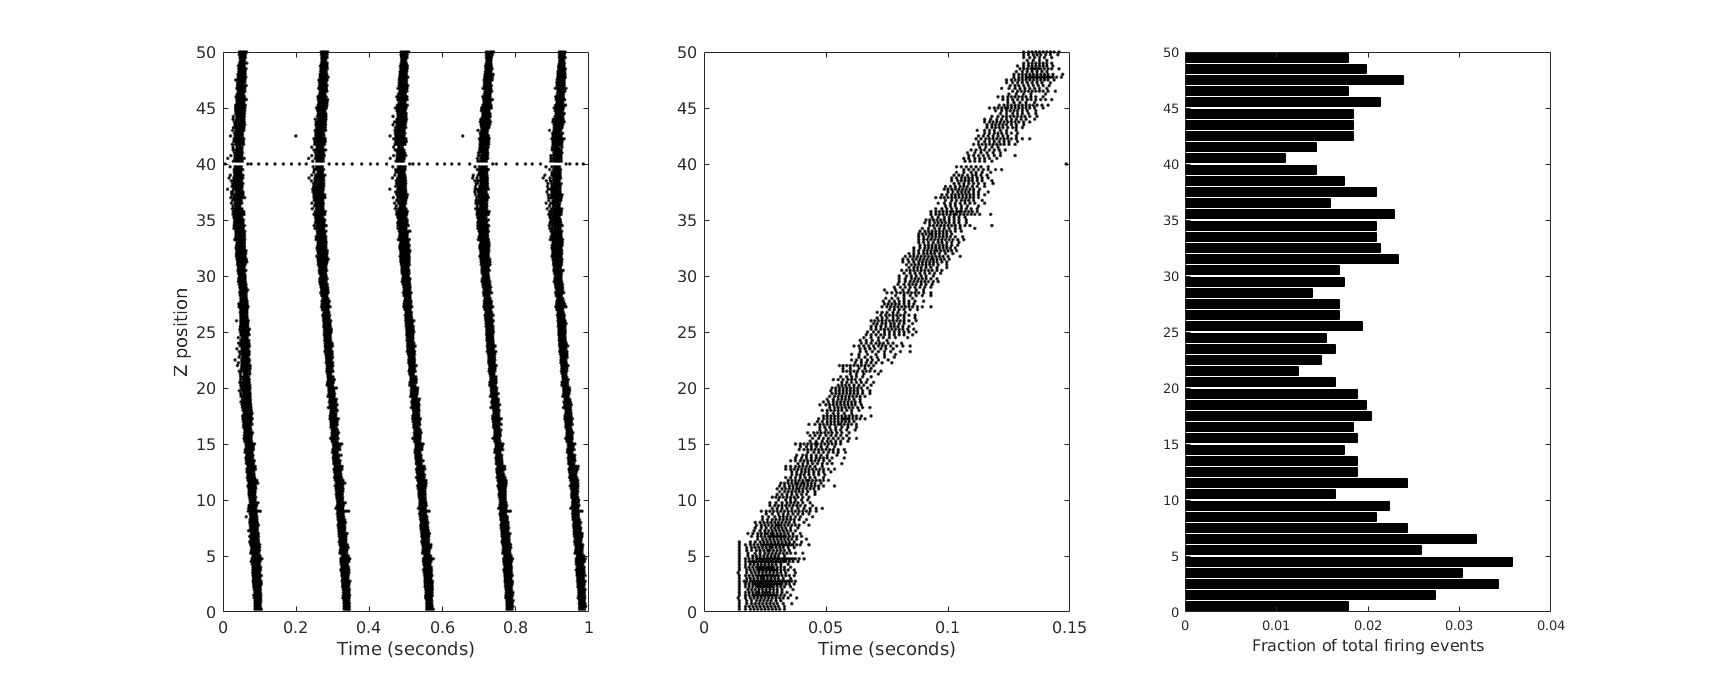
\includegraphics[width=\textwidth]{fig/SingleLTSInhibit}
\end{figure}


\section{Discussion}
We have demonstrated that representative neural structures can support traveling waves in one dimension.
Various parameters determine traveling wave formation and propagation including the connectivity, connection strength, excitatory/inhibitory balance and action potential propagation delay.
Columns with local connectivity support traveling waves, consistent with other simulations and experimental studies of cortical traveling waves.
We have also shown that  a fully-connected column exhibits traveling waves if the action potential propagation time depends on the inter-neuron distance. 
The traveling waves observed with these two types of neuron connectivity correspond to classes of traveling waves proposed in \cite{ermentrout2001}.
The traveling waves in locally connected networks are "Propagating pulses in an excitable network", while the traveling waves in the fully connected network are "Delayed oscillations from a single oscillator" (Figure 1 of \cite{ermentrout2001}).

In \cite{muller2018} the authors noted that mesoscopic traveling waves typically have propagation speeds from 0.1 to 0.8 meters per second, consistent with the axonal conduction speed of unmyelinated fibers.
Our linear model of synaptic conduction delay is linear with inter-neuron distance, so we expected longer synaptic conduction delays to result in slower wave propagation.
The column topology can also influence the propagation speed.
Columns with a larger cross-section have a larger number of neurons and synapses for a given length, providing more pathways for the traveling wave to propagate.
The propagation delay parameter $\kappa$ does effect the wave propagation as expected, but the effect is not linear.
If the traveling wave velocity was determined by the action potential propagation speed we would expect to see wave velocity of 1000 units/second with $\kappa=1$.
Instead the wave velocity is less than half the simple prediction (Figure \ref{fig:delay_topology}).
A four-fold increase in $\kappa$ does not reduce the traveling wave propagation speed by a factor of 4. 

The column topology also has a significant impact on wave propagation speed, with waves in the thinner 2x2 columns traveling about $25\%$ slower than in the 3x3 column.
Real neural minicolumns will have a less regular structure and we may expect them to show a more continuous variation in wave propagation speed. 
The variations in propagation speed could be an important feature of traveling waves in organizing cortical activity.

Our model shows preferential sites for wave initiation due to the presence of inhibitory neurons with low spiking thresholds.
Low-threshold inhibitory neurons in the Izhikevich model represent the low-threshold spiking inhibitory neurons that are found in the cortex \cite{izhikevich2003}\cite{gibson2009}.
These low-threshold neurons could act as ''pacemakers'' for traveling waves, providing spatial and temporal synchronization.

\clearpage
\printbibliography

\end{document}
